\documentclass[12pt,a4paper,titlepage,headinclude,bibtotoc]{scrartcl}

%---- Allgemeine Layout Einstellungen ------------------------------------------

% Für Kopf und Fußzeilen, siehe auch KOMA-Skript Doku
\usepackage[komastyle]{scrpage2}
\pagestyle{plain}
\setheadsepline{0.5pt}[\color{black}]
\automark[section]{chapter}


%Einstellungen für Figuren- und Tabellenbeschriftungen
\setkomafont{captionlabel}{\sffamily\bfseries}
\setcapindent{0em}


%---- Weitere Pakete -----------------------------------------------------------
% Die Pakete sind alle in der TeX Live Distribution enthalten. Wichtige Adressen
% www.ctan.org, www.dante.de

% Sprachunterstützung
\usepackage[ngerman]{babel}

% Benutzung von Umlauten direkt im Text
% entweder "latin1" oder "utf8"
\usepackage[utf8]{inputenc}

% Pakete mit Mathesymbolen und zur Beseitigung von Schwächen der Mathe-Umgebung
\usepackage{latexsym,exscale,stmaryrd,amssymb,amsmath}


\usepackage[nointegrals]{wasysym}
\usepackage{eurosym}

% Anderes Literaturverzeichnisformat
%\usepackage[square,sort&compress]{natbib}
\usepackage{hyperref}
% Für Farbe
\usepackage{color}
\usepackage{graphicx}
\usepackage{wrapfig}
\usepackage{subfigure}

% Caption neben Abbildung
\usepackage{sidecap}


% Befehl für "Entspricht"-Zeichen
\newcommand{\corresponds}{\ensuremath{\mathrel{\widehat{=}}}}
% Befehl für Errorfunction
\newcommand{\erf}[1]{\text{ erf}\ensuremath{\left( #1 \right)}}


%Fußnoten zwingend auf diese Seite setzen
\interfootnotelinepenalty=1000

%Für chemische Formeln (von www.dante.de)
%% Anpassung an LaTeX(2e) von Bernd Raichle
\makeatletter
\DeclareRobustCommand{\chemical}[1]{%
  {\(\m@th
   \edef\resetfontdimens{\noexpand\)%
       \fontdimen16\textfont2=\the\fontdimen16\textfont2
       \fontdimen17\textfont2=\the\fontdimen17\textfont2\relax}%
   \fontdimen16\textfont2=2.7pt \fontdimen17\textfont2=2.7pt
   \mathrm{#1}%
   \resetfontdimens}}
\makeatother
\usepackage{textcomp}
\usepackage{upgreek}
%\begin{document}
%$\upmu$
%\end{document}
%Honecker-Kasten mit $$\shadowbox{$xxxx$}$$
\usepackage{fancybox}

%SI-Package
\usepackage{siunitx}

%keine Einrückung, wenn Latex doppelte Leerzeile
\parindent0pt

%Bibliography \bibliography{literatur} und \cite{gerthsen}
%\usepackage{cite}
\usepackage{babelbib}
\selectbiblanguage{ngerman}

\usepackage{siunitx}
%\begin{document}
 % \SI{1.55}{\micro\metre}
\sisetup{math-micro=\text{µ},text-micro=µ}
\usepackage{amsmath}

\usepackage[verbose]{placeins}
%für \FloatBarrier

\begin{document}

\begin{titlepage}
\centering
\textsc{\Large Physikalisch- Chemisches Grundpraktikum\\[1.5ex] Universität Göttingen}

\vspace*{0.5cm}

\rule{\textwidth}{1pt}\\[0.5cm]
{\huge \bfseries
  Versuch 2: \\[1.5ex]
  Molare Wärmekapazität von Festkörpern }\\[0.5cm]
\rule{\textwidth}{1pt}

\vspace*{0.5cm}


\begin{Large}
\begin{tabular}{ll}
Durchführende: &  Isaac Maksso, Julia Stachowiak\\
Assistent: & Sven Meyer \\
 Versuchsdatum: & 10.11.2016\\
 Datum der ersten Abgabe: & 17.11.2017\\
\end{tabular}
\end{Large}

\vspace*{0.5cm}


\begin{table}[h!]
\centering
\caption{Ergebnisse des Versuchs.}
\begin{tabular}{l|c|c}
Messgröße& Ergebniss&Literaturwert\\
\hline
$\text{T}_{\text{m}}^{\text{RECH}}$&379.0 ± 27.5\;K&493.65\;K\\
$\text{T}_{\text{m}}^{\text{y-Ab}}$&475.9 ± 34.5\;K&\\
$\text{T}_{\text{m}}^{\text{Vant}}$&491.9 ± 35.7\;K&\\
$\text{T}_{\text{m}}^{\text{Graph}}$&471 ± 10\;K&\\
\end{tabular}
\end{table}
\end{titlepage}


\tableofcontents

\newpage


\section{Experimentelles}
\subsection{Experimenteller Aufbau}
\begin{figure}[h]
\centering
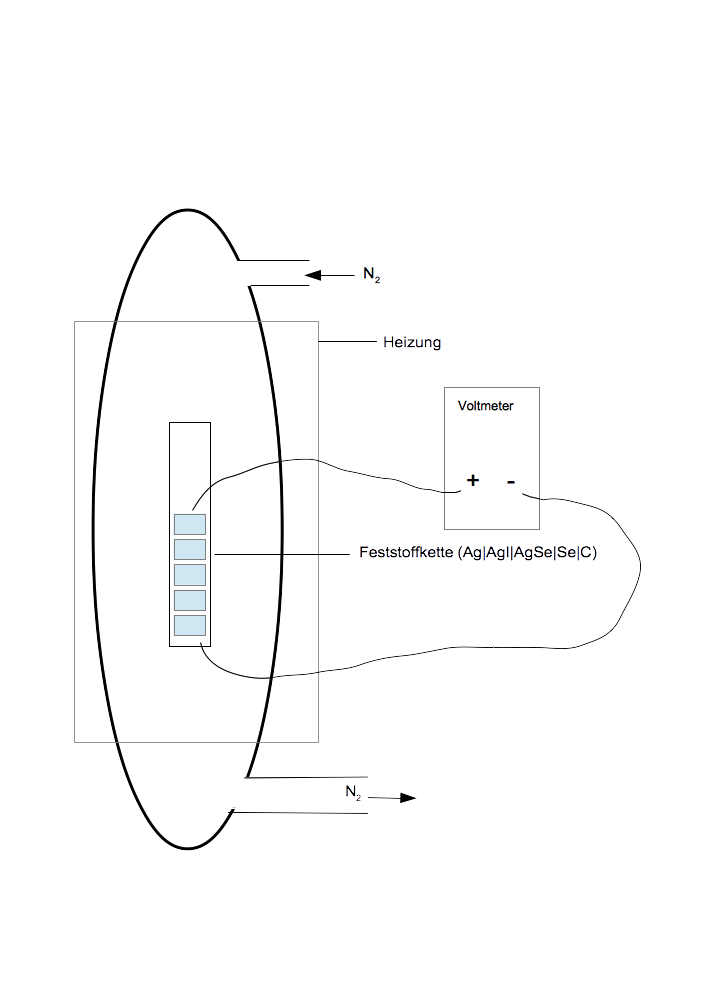
\includegraphics[width=10cm]{VB.png}
\caption{Der Versuchsaufbau.}
\end{figure} 
\FloatBarrier
\subsection{Durchführung}
Es wurde 0.4002\;g Silberiodid abgewogen und zu einer Tablette gepresst. Es wurde eine Feststoffkette, wie in Abbildung 1 zu sehen ist, aufgebaut und 10\;min mit $\text{N}_2$-Gas umspült. Die Feststoffkette wurde auf 160\;°C hochgeheizt und 45\;min bei einem Strom von 1.2\;mA aufgeladen. Es wurde ab 160\;°C in 5\;°C-Schritten die Spannung gemessen. Ab 175\;°C wurde das Messgerät kurzgeschlossen und die Messung fortgesetzt. 
\section{Auswertung}
\subsection{Messergebnisse}
In der Tabelle 2 sind die Messergebnisse der Elektromotorischenkraft dargestellt.
\begin{table}[h!]
\centering
\caption{Messergebnisse des Versuchs.}
\begin{tabular}{c|c||c|c}
T/\;K & EMK/\;V &T/\;K & EMK/\;V\\ 
\hline
433.7 & 0,2889 &   488.15 &0,2860\\ 
438.5 & 0,2871 & 493.15&0,2868 \\
443.25 & 0,2772 &  498.15&0,2877\\
448.15 & 0,2782 & 503.15& 0,2885\\
453.15 &0,2792 & 508.15 &0,2893\\
458.15 & 0,2803 & 513.15 &0,2900\\
463.15 &0,2814 & 518.15 &0,2903\\
468.15 &0,2826 & 523.15&0,2916\\
473.15 &0,2838 & 528.15 & 0,2923\\
478.15 & 0,2844 & 533.15& 0,2933\\
483.15 & 0,2852 &&\\
\end{tabular} 
\end{table}
\FloatBarrier
\subsection{$\Delta_R G$(T) gegen T}
Die freie Reaktionsenergie $\Delta_R G$ lässt sich nach Gl. 1 erechnen:
\begin{align}
\Delta_R G &= - z F \Delta E 
\end{align}
$\Delta E$ berechnet sich folgendermaßen:
\begin{align}
\Delta E &= \Delta E^0 + z\cdot F \cdot \frac{\text{a}(\text{Ag}_2\text{Se})}{\text{a}(\text{Ag})^2\cdot\text{a}(\text{Se})}\\
\Delta E &= \Delta E^0 + R\cdot T\cdot \text{ln}(\frac{1}{1^2\cdot1})\\
\Delta E &= \Delta E^0 + RT \cdot \text{ln}(1)\\
\Delta E &= \Delta E^0 \\
\end{align}
Da die Aktivität von Feststoffen 1 ist, fällt der logorithmische Term weg und Die EMK ist gleich dem Standardelektrodenpotential.\\
Die Werte für $\Delta_R G$ (T) sind in der Tabelle~3 dargestellt.
\begin{table}[h!]
\centering
\caption{Ergebnisse für $\Delta_R G$.}
\begin{tabular}{c|c||c|c}
T/\;K & $\Delta_R G$/\;$\frac{\text{kJ}}{\text{mol}}$ &T/\;K & $\Delta_R G$/\;$\frac{\text{kJ}}{\text{mol}}$\\ 
\hline
433.7 & -55.75 &488.15 & -55.19 \\ 
438.5 & -57.33 & 493.15& -55.52 \\
443.25 & -55.42 &  498.15& -55.67\\
448.15 & -53.68 & 503.15&  -55.83\\
453.15 & -53.88 & 508.15 & -55.96\\
458.15 & -54.09 & 513.15 & -56.12\\
463.15 & -54.30 & 518.15 & -56.12\\
468.15 & -54.53 & 523.15& -56.27\\
473.15 & -54.77 & 528.15 & -56.41\\
478.15 & -54.88 & 533.15& -56.60\\
483.15 & -55.04 &&\\
\end{tabular} 
\end{table}
\FloatBarrier
Der Fehler der freien Reaktionsenthalpie $\Delta(\Delta_R G)$  wird mittels Fehlerfortpflanzung berechnet. Bei den ersten drei Messungen schwankte die Anzeige auf dem Voltometer. Es wurde die Schwankung als Fehler notiert. Ab der vierten Messung konnte die EMK ohne Schwankungen abgelesen werden. Der Fehler wird 0,0005 V:
\begin{align}
\Delta(\Delta_R G)= \sqrt{(-z\cdot F \cdot \Delta(\Delta E))^2}
\end{align}
\begin{table}[h]
\centering
\caption{Fehler für $\Delta_R G$.}
\begin{tabular}{c|c|c}
Temperatur/ K & $\Delta(\Delta E)$/ V & $\Delta(\Delta_R G)$/\;$\frac{\text{kJ}}{\text{mol}}$ \\
\hline
433.7 &  0.005 &  0.1  \\
438.5 & 0.003   & 0.06 \\
443.25 & 0.003  & 0.06 \\
448.15 &  0.0005& 0.01 \\
453.15 & 0.0005& 0.01 \\
458.15 &  0.0005& 0.01 \\
463.15 & 0.0005& 0.01 \\
468.15 & 0.0005& 0.01 \\
473.15 & 0.0005& 0.01 \\
478.15 & 0.0005& 0.01 \\
483.15 & 0.0005& 0.01 \\
488.15 & 0.0005& 0.01 \\
493.15 & 0.0005& 0.01 \\
498.15 & 0.0005& 0.01 \\
503.15 & 0.0005& 0.01 \\
508.15 & 0.0005& 0.01 \\
513.15 & 0.0005& 0.01 \\
518.15 & 0.0005& 0.01 \\
523.15 & 0.0005& 0.01 \\
528.15 & 0.0005& 0.01 \\
533.15 & 0.0005& 0.01 \\
\end{tabular}
\end{table}
\FloatBarrier
\subsection{$\Delta E$ gegen T}
Es wurden die Werte für $\Delta E$ und T aus Tabelle~2 mit den Fehlern aus für $\Delta E$ aus Tabelle~3 aufgetragen in Abbildung~2 aufgetragen. Die Temperatur wurde als fehlerfrei angenommen, da diese nach einer langen Aufheizphase durch kleine Temperaturerhöhungen mittels Thermodingsbums eingestellt wurde. Es wurden bei der linearen Regression die ersten drei Messpunkte nicht eingefügt, da sie sehr stark von den folgenden Messwerten abweichen. 
\begin{figure}[h]
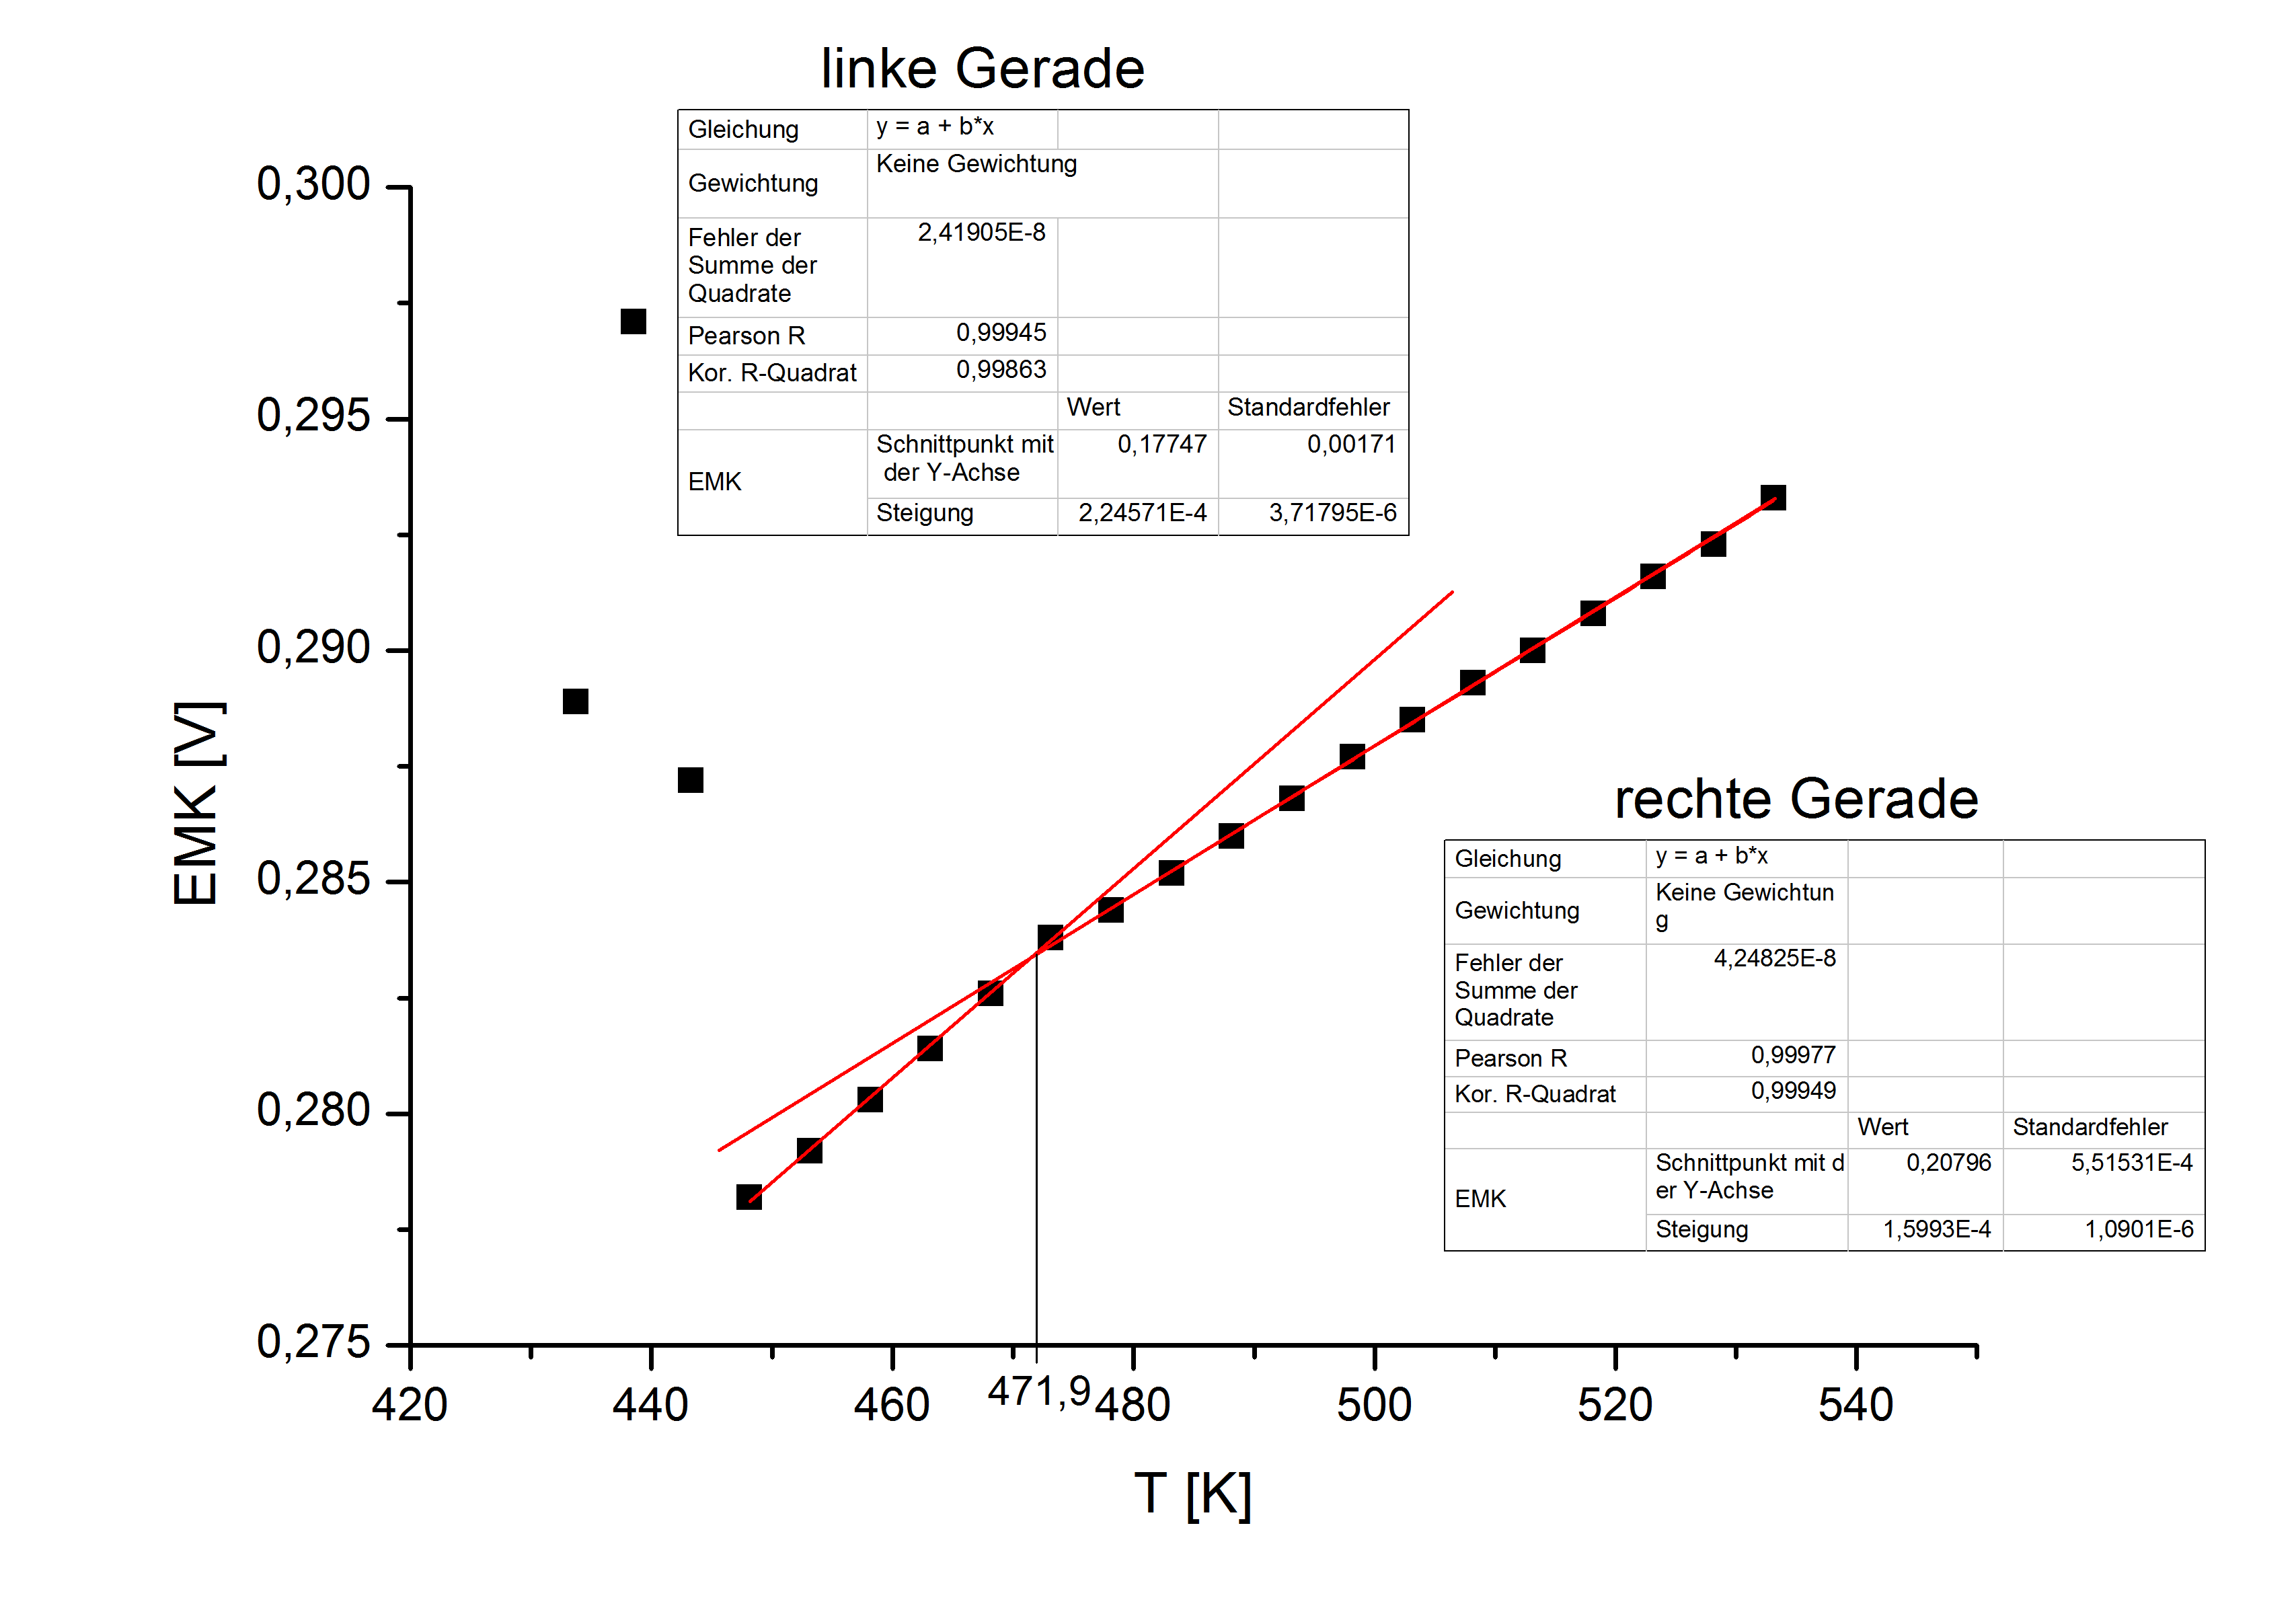
\includegraphics[width=13.5cm]{EMK_gegen_T.png}
\caption{$\Delta E$ gegen T.}
\end{figure} 
\FloatBarrier
Die negative Ableitung der freien Reaktionsentalpie nach der Temperatur ist gleich der Reaktionsentropie. Durch einsetzen der Gleichung~1 wird die Formel zur Berechnung der Reaktionsentropie erhalten. 
\begin{align}
\Delta_R S &= -(\frac{\partial \Delta_R G}{\partial T})\\
&= z \cdot F \cdot (\frac{\partial \Delta E}{\partial T})\\
&= z \cdot F \cdot m \\
\Delta_R S_{\text{s}} &= 2 \cdot 9.6485 \cdot 10^4\;\text{As} \cdot 2.24 \cdot 10^{-4}\;\frac{\text{J}}{\text{K}\cdot\text{mol}}\\
&= 43.3\;\frac{\text{J}}{\text{K}\cdot\text{mol}}\\
\Delta_R  S_{\text{l}} &= 2 \cdot  9.6485 \cdot 10^4\;\text{As} \cdot 1.60 \cdot 10^{-4}\;\frac{\text{J}}{\text{K}\cdot\text{mol}}  \\
&= 30.9\;\frac{\text{J}}{\text{K}\cdot\text{mol}}
\end{align}
Der Fehler der Reaktionsentropie lässt sich mittels Fehlerfortpflanzung berechnen. Der Fehler der Steigung wird hierbei aus dem Auswertungsblatt des Programms $Origin 8.5 G$ entnommen. 
\begin{align}
\Delta(\Delta_R  S)&= \sqrt{(z\cdot F \cdot \Delta m)^2}\\
\Delta(\Delta_R  S_{\text{s}})&= \sqrt{(2\cdot 9.6485 \cdot 10^4\;\text{As} \cdot 0.04 \cdot 10^{-4}\;\frac{\text{J}}{\text{K}\cdot\text{mol}})^2}\\
&= 0.7 \;\frac{\text{J}}{\text{K}\cdot\text{mol}}\\
\Delta(\Delta_R  S_{\text{l}})&= \sqrt{(2\cdot 9.6485 \cdot 10^4\;\text{As} \cdot 0.01\cdot 10^{-4}\;\frac{\text{J}}{\text{K}\cdot\text{mol}})^2}\\
&= 0.2\;\frac{\text{J}}{\text{K}\cdot\text{mol}}
\end{align}
\subsection{Bestimmung der Reaktionsenthalpie}
Aus der Gibbs-Helmholtz-Gleichung ergibt sich die Reaktionsentalpie:
\begin{align}
\Delta_R H=& \Delta_R G +\text{T} \cdot \Delta_R S
\end{align}
Die Ungenauigkeit lässt sich durch die Fehlerfortpflanzung ermitteln. Es wurde für $\Delta(\Delta_R G)$ die Werte aus Tabelle\;4 und für $\Delta(\Delta_R S)$ die Fehler aus Gl.\;12 oder 14 benutzt:
\begin{align}
\Delta(\Delta_R  H)&= \sqrt{(\Delta(\Delta_R G))^2 + (\Delta(\Delta_R S) \cdot \text{T})^2 +(\Delta\text{T} \Delta_R S)^2}\\
\end{align}
\begin{table}[h]
\centering
\caption{Fehler für $\Delta_R G$.}
\begin{tabular}{c|c|c|c|c}
Temperatur/ K & $\Delta$T/ K&Aggregatszustand&$\Delta_R H$/ \;$\frac{\text{kJ}}{\text{mol}}$ & $\Delta(\Delta_R H)$/ \;$\frac{\text{kJ}}{\text{mol}}$ \\
\hline
433.7 &  0.05 &  s. & -37.0 & 1.0\\
438.5 & 0.05   & s. & -38.3 &0.7 \\
443.25 & 0.1  & s. & -36.2&0.7\\
448.15 &  0.05& s. &-34.3&0.3\\
453.15 & 0.05& s. &-34.2&0.3\\
458.15 & 0.05& s. &-34.2&0.3\\
463.15 & 0.05& s. &-34.2&0.3\\
468.15 & 0.05& s. &-34.2&0.3\\
473.15 & 0.05& l. &-40.2&0.1\\
478.15 & 0.05& l. &-40.1&0.1\\
483.15 & 0.05& l. &-40.1&0.1\\
488.15 & 0.05& l. &-40.1&0.1\\
493.15 & 0.05& l. &-40.3&0.1\\
498.15 & 0.05& l. &-40.3&0.1\\
503.15 & 0.05& l. &-40.3&0.1\\
508.15 & 0.05& l. &-40.3&0.1\\
513.15 & 0.05& l. &-40.3&0.1\\
518.15 & 0.05& l. &-40.1&0.1\\
523.15 & 0.05& l. &-40.1&0.1\\
528.15 & 0.05& l. &-40.1&0.1\\
533.15 & 0.05& l. &-40.1&0.1\\
\end{tabular}
\end{table}
\FloatBarrier
Die Werte sind von 433.7\;K bis 468.15\;K und 473.15\;K bis 533.15\;K nahezu konstant. Es wird aufgrunddessen der Mittelwert gebildet, um die Reaktionsenthalpie der festen beziehungsweise flüssigen Phase zu bestimmen. Die Ungenauigkeit wird auch gemittelet:
\begin{align}
\Delta_R H_{\text{x}}&= \frac{1}{n}  \sum_{n=i}^i \Delta_R H_i  \\
\Delta_R H_{\text{s}}&= -35.3 \pm 0.5\;\frac{\text{kJ}}{\text{mol}}\\
\Delta_R H_{\text{l}}&= -40.2 \pm 0.2\;\frac{\text{kJ}}{\text{mol}}
\end{align}
Es ist möglich die Reaktionsenthalpie aus der Auftragung EMK gegen T zu bestimmen. Hierbei erden die Ausdrück für die freie Reaktionsenthalpie und Reaktionsentropie aus der Gleichung \;20 durch die Ausdrücke aus Gleichung\;9 und 1 ersetzt:
\begin{align}
\Delta_R H=&  - z\cdot F \cdot\Delta E +  z \cdot F \cdot (\frac{\partial \Delta E}{\partial T})\cdot\text{T} \\ 
\Delta_R H(0)=&  - z\cdot F\cdot \Delta E(0) +  z \cdot F \cdot (\frac{\partial \Delta E}{\partial T})\cdot 0\\ 
\Delta_R H(0)=&  - z\cdot F \cdot\Delta E(0)
\end{align}
Die Werte für $\Delta E(0)$ wurde aus der Auftragung\;1 abgelesen. 
\begin{align}
\Delta_R H_{\text{s}}=& -34.2\;\frac{\text{kJ}}{\text{mol}}\\
\Delta_R H_{\text{l}}=&  -40.1\;\frac{\text{kJ}}{\text{mol}}
\end{align}
Die Ungenauigkeit wurde mittels Fehlerfortpflanzung bestimmt. Der Fehler des y-Achsenabschnitts wurde aus dem Analysedataenblatt des Zeichenprogramms entnommen.
\begin{align}
\Delta(\Delta_R H)=& \sqrt{(- z\cdot F \cdot\Delta(\Delta E(0)))^2}\\
\Delta(\Delta_R H_{\text{s}})&  0.4\;\frac{\text{kJ}}{\text{mol}}\\
\Delta(\Delta_R H_{\text{l}})=&  0.1\;\frac{\text{kJ}}{\text{mol}}
\end{align}
\section{Auftragung nach Vant'Hoff}
Zwischen der Gleichgewichtskonstante und der freien Reaktionsenthalpie besteht folgender Zusammenhang:
\begin{align}
\text{K}&=e^{\frac{\Delta_R G}{RT}}
\end{align}
In Gl.\;28 wird Gl.\;1 eingesetzt und der natürliche Logorithmus gezogen:
\begin{align}
\text{K}&=e^{\frac{-zF\Delta E}{RT}}\\
\text{ln(K)}&=\frac{-zF\Delta E}{RT}
\end{align}
Die Reaktionsenthalpie kann durch die Vant'Hoff Gleichung aus der Steigung ermittelt werden. Die Wert der aufgetragenen Punkte sind in Tabelle\;6 aufgelistet. Die Steigung wurde aus der Abbildung\;3 abgelesen
\begin{align}
\Bigl(\frac{\text{K}}{\text{T}^{-1}}\Bigr)_p&=\frac{-\Delta_R H}{R}\\
\Delta_R H&=- \Bigl(\frac{\text{K}}{\text{T}^{-1}}\Bigr)_p\cdot R\\
\Delta_R H&=- m_x\cdot R\\
\Delta_R H_{\text{s}}&=-40.4\;\frac{\text{kJ}}{\text{mol}}\\
\Delta_R H_{\text{l}}&=-34.3\;\frac{\text{kJ}}{\text{mol}}\\
\end{align}
\begin{table}[h]
\centering
\caption{Wert für die Auftragung nach Van't Hoff.}
\begin{tabular}{c|c|c}
$\frac{1}{\text{T}}$/ $10^{-3}\frac{1}{\text{K}}$ &Aggregatszustand& ln(K) \\
\hline
2.31 &  s. & 15.5\\
2.28 & s. & 15.7 \\
2.26 & s. &15.0\\
2.23 & s. &14.4\\
2.21 & s. &14.3\\
2.18 & s. &14.2\\
2.16 & s. &14.1\\
2.14 & s. &14.0\\
2.11 & l. &13.9\\
2.10 & l. &13.8\\
2.07 & l. &13.7\\
2.05  & l. &13.6\\
2.03 & l. &13.5\\
2.01 & l. &13.4\\
1.99 & l. &13.3\\
1.97 & l. &13.2\\
1.95 & l. &13.2\\
1.93 & l. &13.0\\
1.91 & l. &12.9\\
1.89 & l. &12.8\\
1.88 & l. &12.8\\
\end{tabular}
\end{table}
\FloatBarrier
\begin{figure}[h]
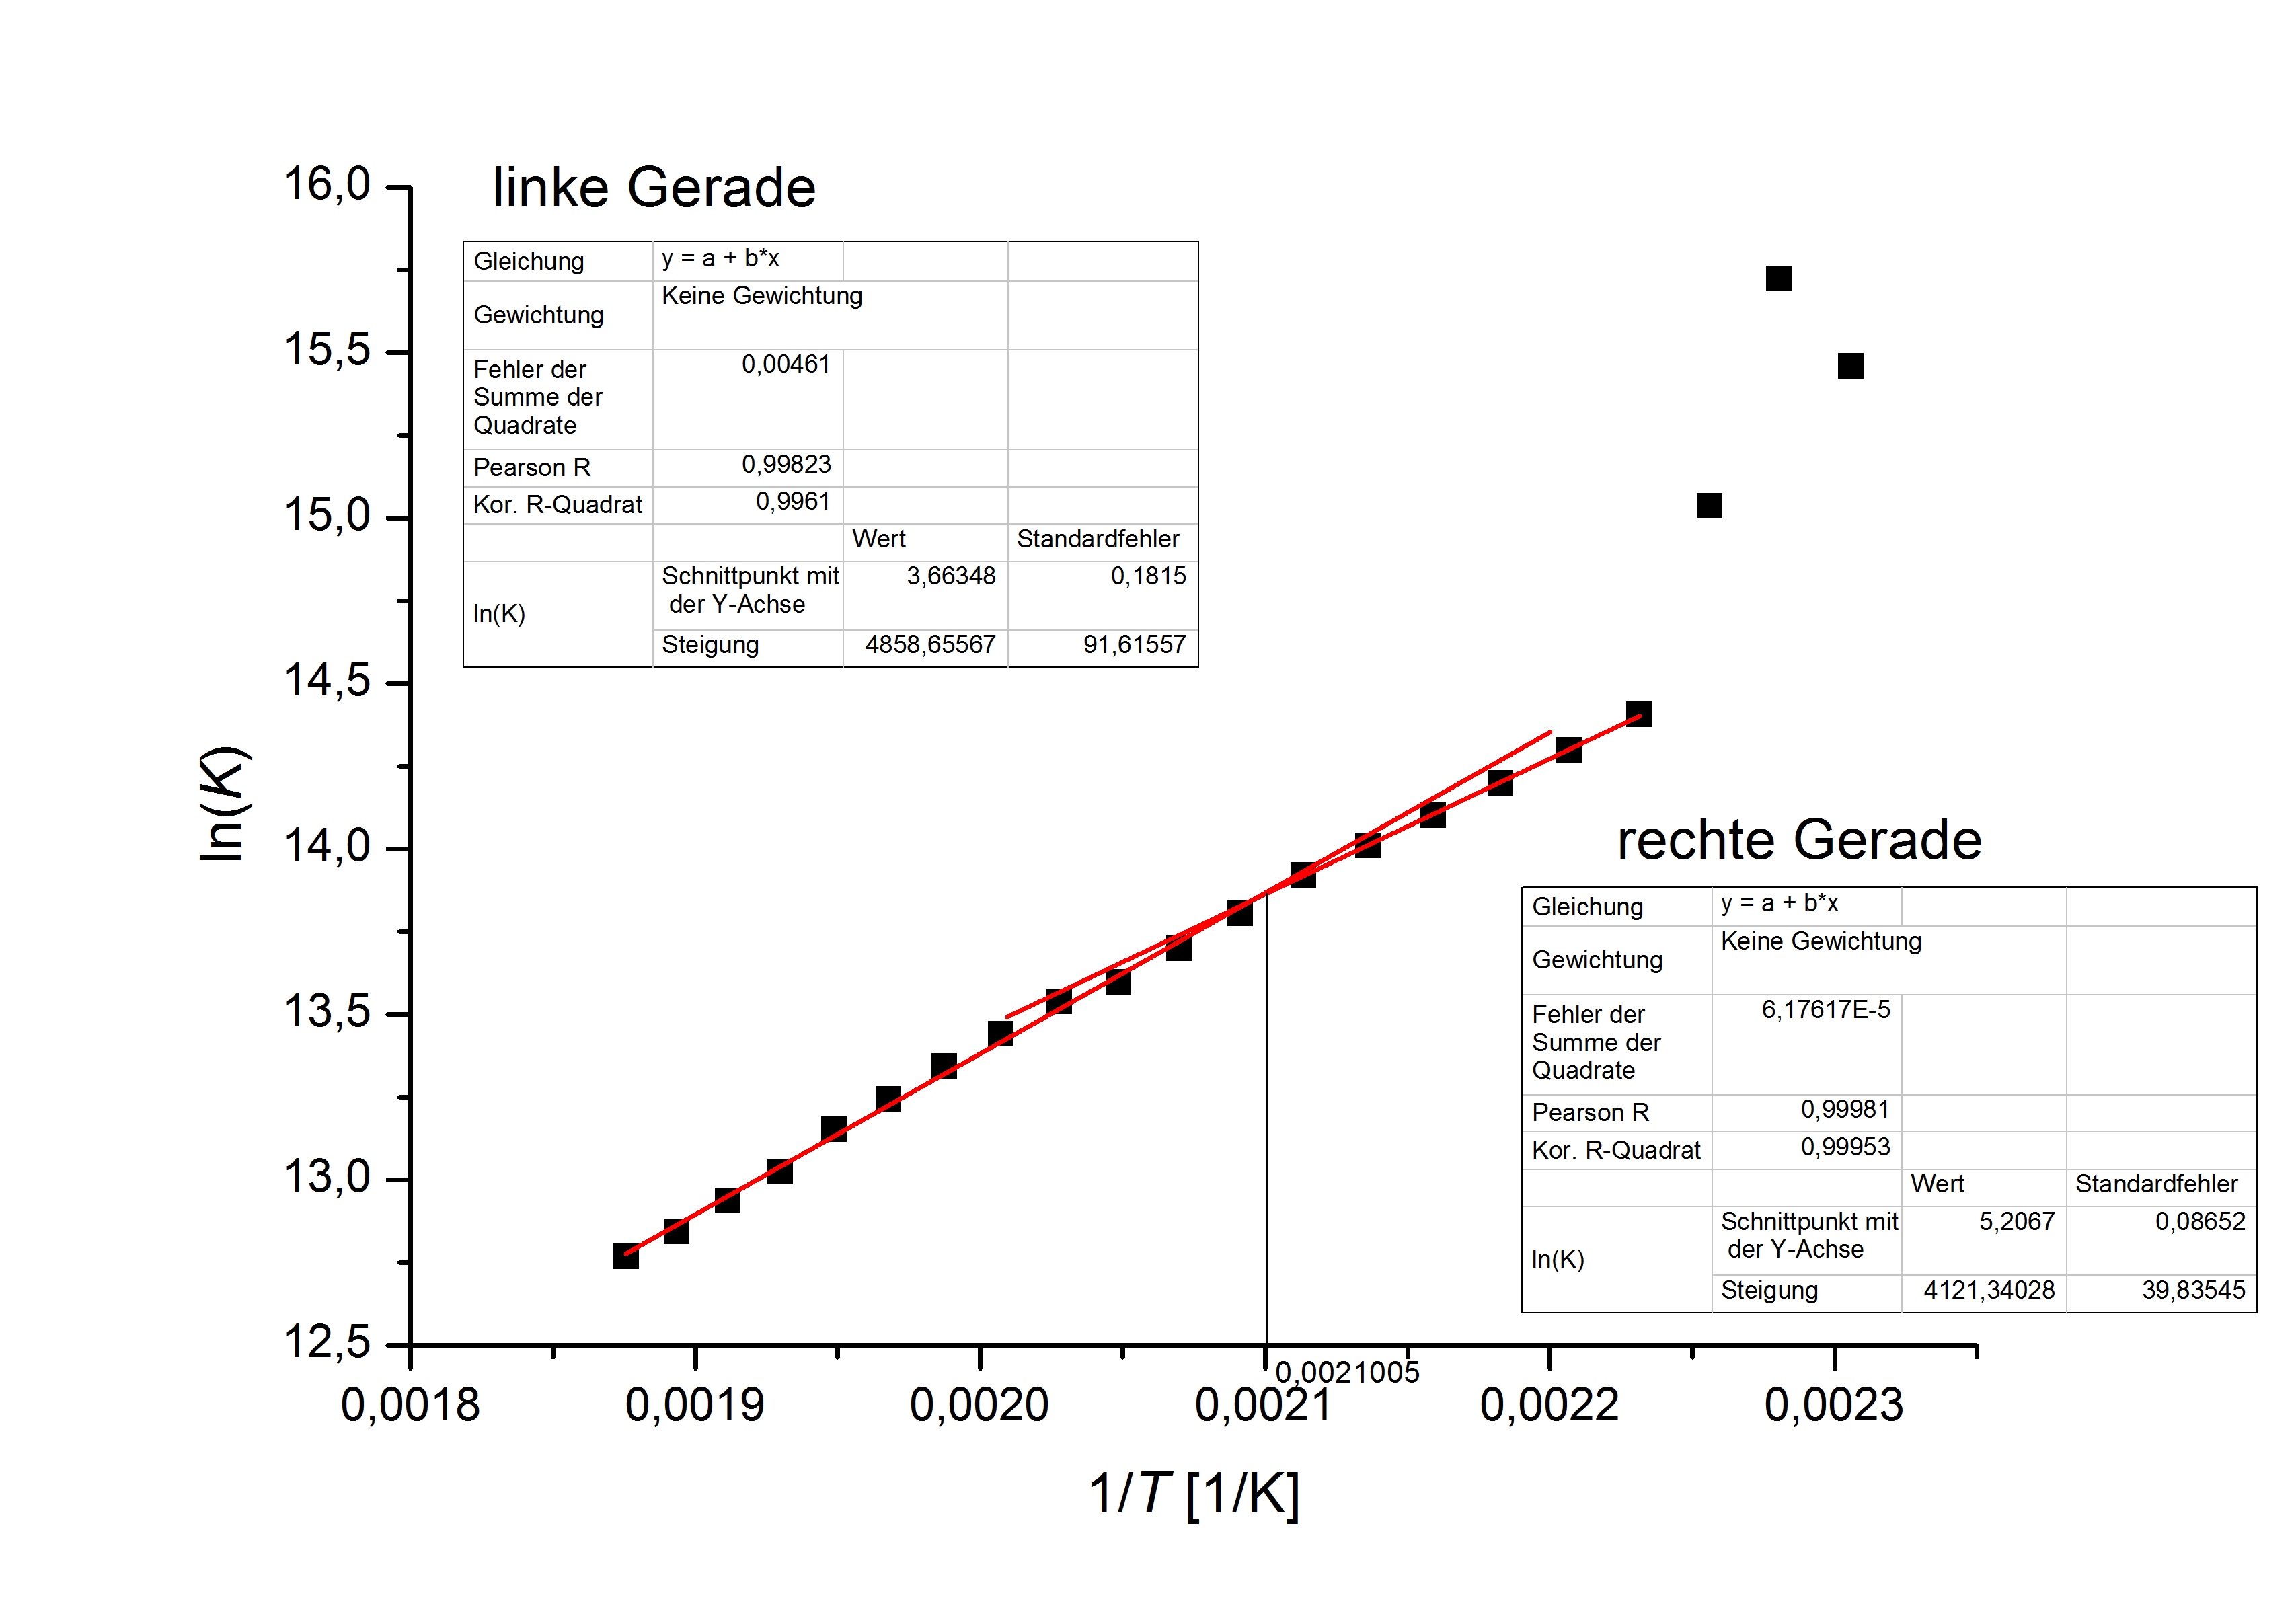
\includegraphics[width=13.5cm]{Van'tHoffAnalogzuEMK.png}
\caption{Auftragung nach Van't Hoff.}
\end{figure} 
\FloatBarrier
Die Ungenauigkeit der Reaktionsenthalpie lässt sich mittels Fehlerfortpflanzung ermitteln. Der Fehler der Steigung wurde aus aus dem Analysdatenblatt der Auftragung entnommen:
\begin{align}
\Delta(\Delta_R H) &= \sqrt{(R\cdot\Delta m)^2}\\
\Delta(\Delta_R H_{\text{s}}) &= 0.8\;\frac{\text{kJ}}{\text{mol}}\\
\Delta(\Delta_R H_{\text{l}}) &= 0.4\;\frac{\text{kJ}}{\text{mol}}
\end{align}
\section{Bestimmung der Umwandlungsenthalpie und Umwandlungsentropie}
Die Umwandungsenthalpie wird aus der Differenz zwischen der Reaktionsenthalpie der festen und der flüssigen Phase bestimmt. Hierbei wird die Unwandlungsenthalpie aus dem Mittelwert der rechenerischen Werte aus Tabelle\;5 ($\Delta_U H_{\text{s}\rightarrow\text{l}}^{\text{RECH}}$) und die Umwandlungsenthalpie aus den y-Abschnitten-Rechnungen Gl.\;26 und 27 ($\Delta_U H_{\text{s}\rightarrow\text{l}}^{\text{y-Ab}}$) berechnet. Die Ungenauigkeit wurde durch Summe der Ungenauigkeit der Reaktionenthalpie in der flüssigen und festen Phase bestimmt:
\begin{align}
\Delta_U H_{\text{s}\rightarrow\text{l}}^{\text{RECH}}=&  -40.2\;\frac{\text{kJ}}{\text{mol}} - \Bigl(-35.3\;\frac{\text{kJ}}{\text{mol}}\Bigr) \pm \Bigl((0.2+0.5)\;\frac{\text{kJ}}{\text{mol}}\Bigr)\\
\Delta_U H_{\text{s}\rightarrow\text{l}}^{\text{RECH}}=& -4.7\pm 0.7 \;\frac{\text{kJ}}{\text{mol}}\\
\Delta_U H_{\text{s}\rightarrow\text{l}}^{\text{y-Ab}}=&  -40.1\;\frac{\text{kJ}}{\text{mol}} - \Bigl(-34.2\;\frac{\text{kJ}}{\text{mol}}\Bigr) \pm \Bigl((0.4+0.1)\;\frac{\text{kJ}}{\text{mol}}\Bigr)\\
\Delta_U H_{\text{s}\rightarrow\text{l}}^{\text{y-Ab}}=& -5.9 \pm 0.5 \;\frac{\text{kJ}}{\text{mol}}\\
\Delta_U H_{\text{s}\rightarrow\text{l}}^{\text{Vant}}=&  -40.4\;\frac{\text{kJ}}{\text{mol}} - \Bigl(-34.3\;\frac{\text{kJ}}{\text{mol}}\Bigr) \pm \Bigl((0.8+0.4)\;\frac{\text{kJ}}{\text{mol}}\Bigr)\\
\Delta_U H_{\text{s}\rightarrow\text{l}}^{\text{Vant}}=& -6.1 \pm 1.2 \;\frac{\text{kJ}}{\text{mol}}
\end{align}
Die Umwandlungsentropie berechnet sich ähnlich der Umwandlungsenthaplie aus der Different der Reaktionsentropien der festen und flüssigen Phase. Die Fehler wurden auch zu Größtfehlern summiert. Es wurden die Werte aus den Gleichungen\;12, 14, 17 und 19 genutzt:
\begin{align}
\Delta_U S_{\text{s}\rightarrow\text{l}}=&  30.9\;\frac{\text{J}}{\text{K}\cdot\text{mol}} - 43.3\;\frac{\text{J}}{\text{K}\cdot\text{mol}} \pm \Bigl((0.7+0.2)\;\frac{\text{J}}{\text{K}\cdot\text{mol}}\Bigr)\\
\Delta_U S_{\text{s}\rightarrow\text{l}}=& -12.4\pm0.9 \;\frac{\text{J}}{\text{K}\cdot\text{mol}}
\end{align}
\section{Schmelzpunktbestimmung}
Ist das System im Phasengleichgewicht ist die freie Reaktionsenthalpie gleich 0. Die Gibbs-Hemlholzgleichung (Gl.\;20) wird kann nach T umgestellt werden. Um die Schmelztemperatur bestimmen zu können wird der Quotient aus der Umwandlungsenthalpie und der Umwandlungsenthropie aufgestellt:
\begin{align}
\text{T}_{\text{m}}= \frac{\Delta_U H_{\text{s}\rightarrow\text{l}}}{\Delta_U S_{\text{s}\rightarrow\text{l}}}
\end{align}
Der Fehler lässt sich mittels Fehlerfortpflanzung bestimmen:
\begin{align}
\text{T}_{\text{m}}= \sqrt{\Bigl(\frac{1}{\Delta_U S_{\text{s}\rightarrow\text{l}}}\cdot \Delta(\Delta_U H_{\text{s}\rightarrow\text{l}})\Bigr)^2+\Bigl(\frac{\Delta_U H_{\text{s}\rightarrow\text{l}}}{(\Delta_U S_{\text{s}\rightarrow\text{l}})^2}\cdot \Delta(\Delta_U S_{\text{s}\rightarrow\text{l}})\Bigr)^2}
\end{align}
In der Tabelle\; sind die bestimmten Schmelztemperatur für die rechnerisch, mit dem y-Achsenabschnitt bestimmten Enthalpie aufgelistet.
\begin{table}[h]
\centering
\caption{Schmelztemperatur durch verschiedene Methoden bestimmt.}
\begin{tabular}{c|c|c}
Methode & $\text{T}_{\text{m}}$/ K& $\Delta\text{T}_{\text{m}}$/ K \\
\hline
RECH &379.0 &27.5 \\
y-Ab&475.8 & 34.5\\
Vant&491.9 & 35.7\\
\end{tabular}
\end{table}
\FloatBarrier
Die Schmelztemperatur kann auch aus der Auftragung EMK gegen T bestimmt werden. Am Schnittpunkt, den die Geraden bilden, wird der x-Achsenwert abgelesen. Der Ablesefehler wird aufgrund der breiten Überschneidung auf 10\;K geschätzt:
\begin{align}
\text{T}_{\text{m}}^{\text{Graph}}&= 471.9 \pm 10\;\text{K}
\end{align}
\section{Diskussion}
\begin{table}[h!]
\centering
\caption{Ergebnisse des Versuchs.}
\begin{tabular}{l|c|c}
Messgröße& Ergebniss&Literaturwert\\
\hline
$\Delta_R S_{\text{l}}$&30.9 ± 0.2\;$\frac{\text{J}}{\text{K}\cdot\text{mol}}$&??? \;$\frac{\text{kJ}}{\text{K}\cdot\text{mol}}$\\
\hline
\text{}\text{}\text{}$\Delta_R S_{\text{s}}$&43.3 ± 0.7\;$\frac{\text{J}}{\text{K}\cdot\text{mol}}$&??? \;$\frac{\text{kJ}}{\text{mol}}$\\
\hline
$\Delta_U S_{\text{s}\rightarrow\text{l}}$&-12.4 ± 0.9\;$\frac{\text{J}}{\text{K}\cdot\text{mol}}$&??? \;$\frac{\text{kJ}}{\text{mol}}$\\
\hline
$\Delta_R H_{\text{l}}^{\text{RECH}}$&-40.2 ± 0.2\;$\frac{\text{kJ}}{\text{mol}}$&??? \;$\frac{\text{kJ}}{\text{mol}}$\\
$\Delta_R H_{\text{l}}^{\text{y-Ab}}$&-34.2 ± 0.1\;$\frac{\text{kJ}}{\text{mol}}$&\\
$\Delta_R H_{\text{l}}^{\text{Vant}}$&-34.3 ± 0.4\;$\frac{\text{kJ}}{\text{mol}}$&\\
\hline
$\Delta_R H_{\text{s}}^{\text{RECH}}$&-35.3 ± 0.5\;$\frac{\text{kJ}}{\text{mol}}$&??? \;$\frac{\text{kJ}}{\text{mol}}$\\
$\Delta_R H_{\text{s}}^{\text{y-Ab}}$&-40.1 ± 0.4\;$\frac{\text{kJ}}{\text{mol}}$&\\
$\Delta_R H_{\text{s}}^{\text{Vant}}$&-40.4 ± 0.8\;$\frac{\text{kJ}}{\text{mol}}$&\\
\hline
$\Delta_U H_{\text{s}\rightarrow\text{l}}^{\text{RECH}}$&-4.7 ± 0.7\;$\frac{\text{kJ}}{\text{mol}}$&??? \;$\frac{\text{kJ}}{\text{mol}}$\\
$\Delta_U H_{\text{s}\rightarrow\text{l}}^{\text{y-Ab}}$&-5.9 ± 0.5\;$\frac{\text{kJ}}{\text{mol}}$&\\
$\Delta_U H_{\text{s}\rightarrow\text{l}}^{\text{Vant}}$&6.1 ± 1.2\;$\frac{\text{kJ}}{\text{mol}}$&\\
\hline
$\text{T}_{\text{m}}^{\text{RECH}}$&379.0 ± 27.5\;K&493.65\;K\\
$\text{T}_{\text{m}}^{\text{y-Ab}}$&475.9 ± 34.5\;K&\\
$\text{T}_{\text{m}}^{\text{Vant}}$&491.9 ± 35.7\;K&\\
$\text{T}_{\text{m}}^{\text{Graph}}$&471 ± 10\;K&\\
\end{tabular}
\end{table}
Es wurden keine Literaturwerte für die Reaktionsentropie, -enthalpie und Umwandlungsenthalpie gefunden. Sie könnten mittels Standardbildungsenthalpiewerten beziehungsweise Standardbildungsentropiewerten über den Satz von Heß berechnet werden. Die Umwandlungsenthalpie/entropie würden ähnlich der Gl.\;46 und 52 bestimmt werden. Es fehlen jedoch die Werte des Silber(I)selenids und des Selens im flüssigen Aggregatzustand. Aus diesem Grund werden nur die Messergebnisse der Schmelztemperatur diskutiert.\\
Die ermittelten Schmelztemperaturen sind alle bis auf $\text{T}_{\text{m}}^{\text{RECH}}$ dem Literaturwert nahe. Die Schmelztemperatur $\text{T}_{\text{m}}^{\text{RECH}}$ liegt unter dem Literaturwert. Ursache hierfür könnte die ersten 3 Messungen sein. Hier sind die bestimmten Reaktionsenthalpien im Vergleich zu den übrigen Messungen 2-4\;$\frac{\text{kJ}}{\text{mol}}$ größer. Die nachfolgenden Messungen schwanken um 0.1\;$\frac{\text{kJ}}{\text{mol}}$, was einen systematischen Fehler bei den ersten 3 Messungen vermuten lässt. Da die Reaktionsentropie ohne die 3 ersten Messungen bestimmt wurde, wird die Abweichung auf die freie Reaktionsenthalpie zurückgeführt. Hier führt eine zu groß bestimmte EMK zu einem höheren Betrag an freier Reaktionsenthalpie führen. Die Messung könnte durch das noch angeschlossen Ladegerät, welches ab der vierten Messung entfernt wurde, verfälscht worden sein.
\newpage
\section{Literaturverzeichnis}
1\quad Lide, D.R.:\textit{CRC Handbook of Chemistry and Physics}, CRC Press LLC, Boca 84. edition, S.4-312, \textbf{2003}.

\vspace{0,5 cm}
\end{document}


	